\section{Zielsetzung}
\label{sec:Ziel}
In diesem Versuch wird das Absorptionsverhalten von $\beta$\,- und $\gamma$\,-Strahlung untersucht. Aus dem Absorptionsverhalten wird dann für $\beta$\,-Strahlung die 
maximale Energie der $\beta$\,- Teilchen bestimmt. Für $\gamma$\,-Strahlung werden die relevanten Größen des exponentiellen Absorptionsgesetzes \ref{eqn:Absorbgesetz} bestimmt.
Gelingt dies wird ebenfalls auf den vorliegenden Absorptionsmechanismus geschlossen.

\section{Theorie}
\label{sec:Theorie}
Für diesen Versuch werden grundlegende Kenntnisse zur Erzeugung und Eigenschaften von $\beta$\,- und $\gamma$\,-Strahlung benötigt. Außerdem muss das Wechselwirkungsverhalten der
beiden verwendeten Strahlungsarten bekannt sein. Diese Themen werden in den folgenden Abschnitten erklärt.

\subsection{Gamma-Strahlung}
\label{subec:Gammastrahlung}
$\gamma$\,-Quanten können entstehen, wenn ein angeregter Atomkern, also ein Atomkern mit erhöhter Energie, in einen niederenergetischen und stabileren Zustand zurückfällt. Die 
dabei entstehende Energiedifferenz wird in Form von $\gamma$\,-Quanten frei. Ein $\gamma$\,-Quant ist allerdings kein Teilchen im klassischem Sinne. Ebenfalls können "einzelne"
$\gamma$\,-Quanten nicht nur durch ihren Wellencharakter beschrieben werden. Wird aber eine große Zahl an $\gamma$\,-Quanten betrachtet kann im zeitlichen Mittel der 
Teilchencharakter vernachlässigt werden. Daher kann $\gamma$\,-Strahlung in diesem Versuch als elektromagnetische Welle, mit den typischen Eigenschaften der e-m-Welle,
betrachtet werden. Daher gilt für $\gamma$\,-Strahlung gemäß der Quantentheorie 
\begin{equation*}
    E_{\gamma} = \frac{h}{\nu} = \frac{hc}{\lambda}.
\end{equation*}
Dabei ist h das Planksche Wirkungsquantum, c die Lichtgeschwindigkeit, $\nu$ die Frequenz und $\lambda$ die Wellenlänge der $\gamma$\,-Strahlung. Das $\gamma$\,-Spektrum ist 
nicht kontinuierlich, sonder sehr diskret. Dies folgt aus der Eigenschaft der Energieniveaus der Kerne, denn die Kernenergieniveaus sind genau definiert.

\subsection{Wechselwirkungsverhalten von Gamma-Strahlung mit Materie}
\label{Gammawechselwirkung}
Trifft ein $\gamma$\,-Quant auf Materie tritt es in Wechselwirkung mit dieser. Dabei kann $\gamma$\,-Quant mit unterschiedlichen Bausteinen der Materie wechselwirken. 
Alle bisher bekannten Wechselwirkungen werden in \autoref{fig:TabelleGamma} dargestellt.

\begin{figure}
    \centering
    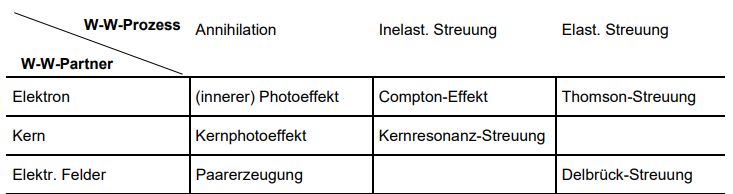
\includegraphics[width = 0.7\textwidth]{content/TabelleGamma.png}
    \caption{In dieser Abbildung ist eine Tabelle der möglichen Wechselwirkungen eines Gamma-Quants mit Materie dargestellt. \cite{v704}.}
    \label{fig:TabelleGamma}
\end{figure}

Aufgrund der Relevanz für diesen Versuch wird nun lediglich auf die dominierenden Wechselwirkungen, im üblichen $\qty{10}{\kilo\electronvolt}$ - $\qty{10}{\mega\electronvolt}$
$\gamma$\,-Energiespektrum, eingegangen. Das sind der Photo-Effekt, der Compton-Effekt und die Paarbildung.


Tritt der (innere) Photoeffekt auf, wechselwirkt ein $\gamma$\,-Quant mit einem Hüllenelektron des Materials. Dadurch wird das $\gamma$\,-Quant annihiliert und Energie und 
Impuls des $\gamma$\,-Quants werden an das Meterial abgegeben. Dabei erhält das Elektron, mit welchem die Wechselwirkung stattfindet die Energie des $\gamma$\,-Quants.
Daher kann die Energie des Elektrons durch 
\begin{equation*}
    E_{\symup{e}} = h\nu - E_{\symup{B}}
\end{equation*}
beschrieben werden. Dabei ist $E_{\symup{B}}$ die Bindungsenergie des Elektrons und $h\nu$ die übertragene Energie des $\gamma$\,-Quants. Gilt nun $h\nu > E_{\symup{B}}$, wird
das Elektron aus der Hülle gelöst(Photoeffekt). Ist jedoch die Bindungsenergie größer ist der Photoeffekt nicht möglich.  Der Impuls des $\gamma$\,-Quants geht dabei auf den 
Atomkern über. Dies geschieht aber nur, wenn das Elektron fest genug an das Atom gebunden ist, woraus folgt das die Wahrscheinlichkeit des Photoeffekts auf inneren 
Elektronenschalen größer ist. Daraus folgt wiederum, dass der Wirkungsquerschnitt, welcher im \autoref{subesc:Wirkungsquerschnitt} erläutert wird, proportional zur fünften 
Potenz der Ordnungszahl und zu $E_\gamma^{-3.5}$ ist.


Der Compton-Effekt beschreibt eine Streuung des $\gamma$\,-Quants an einem freien Elektron. Im gegensatz zum Photoeffekt, wo das $\gamma$\,-Quant annihiliert wird, kann ein 
$\gamma$\,-Quant nicht seine gesamte Energie an ein freies Elektron abgeben. Daher bleibt bei dem Comptoneffekt immer ein $\gamma$\,-Quant erhalten. Durch die Energie- und 
Impuls-Übertragung des $\gamma$\,-Quants an das Elektron ändert sich aber die Richtung und Intensität des $\gamma$\,-Quants. 

Für die Paarbildung muss die Energie des $\gamma$\,-Quants größer als die dopellte Ruhemasse des Elektrons sein. Ist diese Energie gegeben kann ein $\gamma$\,-Quant unter 
Kollision annihiliert werden und somit ein Elektron und ein Positron bilden. Dabei wird ein gewisser Impuls an den Stoßpartner übertragen.

Für diese drei Effekte besteht allerdings keine diskrete Energieaufteilung. Allerdings unterliegt die Wahrscheinlichkeit der Effekte unteschiedlichen Energie- und 
Ordnungszahlabhängigkeiten. Daher kann zu einer gegebenen Ordnungszahl eine Verteilungskurve der Effekte abhängig von der Energie erstellt werden.

Für kleine Ordnungszahlen dominiert bei kleinen Energien der Photoeffekt. Ab $\qty{200}{\kilo\electronvolt}$ übernimmt dann hauptsächlich der Comptoneffekt. Mit steigender 
Energie ab $\qty{1}{\mega\electronvolt}$ setzt die Paarbildung ein. Ab circa $\qty{5}{\mega\electronvolt}$ findet praktisch ausschließlich Paarbildung statt.

\subsection{Beta-Strahlung}
\label{subsec:Betastrahlung}
$\beta$\,-Teilchen können in instabilen Atomkernen entstehen. Dabei kann ein Neutron in ein Proton, ein $\beta^+$\,-Teilchen und ein Antielektronenneutrino oder
ein Proton in ein Neutron, ein $\beta^-$\,-Teilchen und ein Elektronenneutrino zerfallen. Die dabei entstehenden $\beta$\,-Teilchen sind positive oder negative schnelle
Elektronen. Da sich die freiwerdene Umwandlungsenergie statistisch auf die entstehenden Teilchen verteilt, entsteht beim $\beta$\,-Strahler ein kontinuierliches Spektrum.

\subsection{Wechselwirkungsverhalten von Beta-Strahlung mit Materie}
\label{BetaWechselwirkung}
Trifft ein $\beta$\,-Teilchen nun auf eine Absorberschicht können im wesentlichen drei dominierende Prozesse auftreten.


Zum einen kann die Rutherford-Streuung auftreten. Diese beschreibt eine elastische Streuung am Atomkern des Absorbermaterials. Dabei werden die $\beta$\,-Teilchen, welche 
als paralleles Strahlenbündel auf das Meterial treffen durch die elektrischen Felder der Atomkerne abgelengt. Dies hat eine breite statistische Verteilung an Richtungen 
zufolge. Außerdem kann es durch diese Streuung passieren, dass die Reichweite $R$ der $\beta$\,-Teilchen nicht mehr ausreicht um wieder aus dem Material auszutreten. 


Des weiteren kann aber auch eine inelastische Streuung an den Atomkernen stattfinden. Durch die Ablenkungen im elektrischen Feld muss Energie abgestrahlt werden. Diese 
Energie wird Bremsstrahlung genannt, weil die $\beta$\,-Teilchen durch die abgestrahlte Energie an Geschwindigkeit verlieren. Die Wahrscheinlichkeit für diesen Prozess
wird durch den Wirkungsquerschnitt
\begin{equation*}
    \sigma_{\symup{Br}} = \alpha r_e^2 z^2
\end{equation*}
beschrieben. Die Energie der Bremsstrahlung kann durch Integration aller Streuwinkel zu 
\begin{equation*}
    E_{\symup{Br}} = 7\cdot 10^{-7} z E_\beta^2
\end{equation*}
berechnet werden. Dabei ist $E_\beta$ die Energie der $\beta$\,-Teilchen. Diese Gleichung gilt nur Näherungsweise für Energien $E_\beta$ bis zu $\qty{2500}{\kilo\electronvolt}$. 
Aus verschiedenen Berchungen zeigt sich, dass diese Form der Energieabgabe nur eine untergeordnete Rolle in der Absorption von $\beta$\,-Teilchen spielt.

Eine weitere Energieabgabe der $\beta$\,-Teilchen liegt in der inelastischen Streuung an Elektronen. Hierbei gibt des $\beta$\,-Teilchen bei jedem Stoß einen kleinen Teil der
Energie ab, wodruch des gestoßene Atom ionisiert wird. Dieser Prozess kann für jedes $\beta$\,-Teilchen häufig auftreten. Die Wahrscheinlichkeit für für diesen Prozess
ist proportional zur Ordnungszahl und zu Anzahl der Atome pro Volumen im Material. Der Energieverlust pro Stoßprozess kann bei $\beta$\,-Teilchen mit Energien kleiner als
$m_0 c^2$ ist durch 
\begin{equation}
    \label{eqn:inelast_elek_everlust}
    \frac{\symup{d}E}{\symup{d}x} = -\frac{2\pi r_e^2}{E_\beta}\frac{N_L\rho}{M}z\symup{ln}\frac{E_\beta}{I}
\end{equation}
beschrieben. Hier beschreibt $I$ die Ionisationsenergie des Absorbermaterials.

\subsection{Wirkungsquerschnitt}
\label{subsec:Wirkungsquerschnitt}
Wie bisher beschrieben treten verschiedene Wechselwirkungen beim Eintreten von Strahlung in Materie auf. Die Häufigkeit dieser Wechselwirkungen pro Teilchen und pro Fläch
wird Wirkungsquerschnitt $\sigma$ genannt.